% ----------
% A LaTeX template for course project reports
% 
% This template is modified from "Tech Report ala MIT AI Lab (1981)"
% 
% ----------
\documentclass[12pt, letterpaper, twoside]{article}
\usepackage{geometry}
\usepackage[utf8]{inputenc}
\usepackage[english]{babel}
\usepackage[runin]{abstract}
\usepackage{titling}
\usepackage{booktabs}
\usepackage{fancyhdr}
\usepackage{helvet}
\usepackage{csquotes}
\usepackage{graphicx}
\usepackage{blindtext}
\usepackage{parskip}
\usepackage{etoolbox}

\documentclass{article}
\usepackage{float} % For H float option
%\input{preamble.tex}

% ----------
% Variables
% ----------

\title{\textbf{ICSHelper}} % Full title of your tech report
%\runningtitle{On Image Matting} % Short title
\author{Ahila, Pawan, Shutong Wu, Yi-Leng Chen \and [rameshra,kumarp40,wu867,cheny997]@mcmaster.ca} % Full list of authors
%\runningauthor{Student Name 3 et al.} % Short list of authors


% ----------
% actual document
% ----------
\begin{document}
\maketitle

\begin{abstract}
    \noindent
    An ICS (iCalendar) file is a universal calendar format utilized by mainstream email and various calendar apps such as Microsoft Outlook, Google Calendar, and Apple Calendar. Importing an ICS file into calendar apps allows for the addition of new schedules comprising one or more events. Currently, the process of manipulating ICS files involves editing schedules within calendar apps and then exporting them. To address this time-consuming task, we propose ICS Helper, a Domain-specific Language (DSL) designed for handling ICS files. The primary features of ICS Helper include generating schedules outside of calendar applications, managing massive schedules and events, and automating workflow processes. With its user-friendly syntax, ICS Helper enables users to manage their schedules more effectively.
\end{abstract}

\vspace{2.5cm}

% Uncomment the following to add thanks.
% {\footnotesize
%     \noindent
%     Special thanks to \textbf{Person 1} and \textbf{Affiliation A} for financial support for this project.
% }

\thispagestyle{firstpage}

\pagebreak
% ----------
% End of first page
% ----------

\newgeometry{} % Redefine geometries (normal margins)

\section{Introduction}
\label{sec:intro}

**will modify the content in the future\\
    An ICS (iCalendar) file is a universal calendar format utilized by mainstream email and various calendar apps such as Microsoft Outlook, Google Calendar, and Apple Calendar. Importing an ICS file into calendar apps allows for the addition of new schedules comprising one or more events. Currently, the process of manipulating ICS files involves editing schedules within calendar apps and then exporting them. To address this time-consuming task, we propose ICS Helper, a Domain-specific Language (DSL) designed for handling ICS files. The primary features of ICS Helper include generating schedules outside of calendar applications, managing massive schedules and events, and automating workflow processes. With its user-friendly syntax, ICS Helper enables users to manage their schedules more effectively.
\newpage
\section{Metamodel Definition and Analysis}

The metamodel defined using Emfatic/Ecore serves as the foundation for the ICS Helper DSL. Below is the metamodel along with an analysis of its components, assumptions, and alternative design considerations.

\subsection{Metamodel Overview}

The metamodel defines the structure and relationships of entities within the ICS Helper DSL. It comprises five main classes: \texttt{Schedule}, \texttt{Location}, \texttt{Organizer}, \texttt{Invitee}, and \texttt{Event}. These classes encapsulate various aspects of scheduling and event management.

\begin{itemize}
    \item \textbf{Schedule}: Represents a schedule containing multiple events. It includes attributes for name and description, along with associations with events and the schedule owner.
    
    \item \textbf{Location}: Represents the physical or virtual location of an event. It contains an attribute for the address.
    
    \item \textbf{Organizer}: Represents the organizer of a schedule or event. It includes attributes for name and email, as well as an association with a location.
    
    \item \textbf{Invitee}: Represents an individual invited to an event. It includes attributes for name and email.
    
    \item \textbf{Event}: Represents a specific event within a schedule. It includes attributes for title, description, start date, end date, and recurrence. It also has associations with attendees, the parent schedule, and the event location.
\end{itemize}

\subsection{Assumptions}

The metamodel assumes certain characteristics of schedules, events, organizers, and invitees:

\begin{itemize}
    \item Events can have multiple attendees.
    \item Events are part of a schedule.
    \item Organizers and invitees have associated email addresses.
    \item Each event has a single location.
\end{itemize}

\subsection{Alternative Design Considerations}

While the current metamodel provides a solid foundation, alternative design considerations could enhance its flexibility and completeness:

\begin{itemize}
    \item Event Recurrence: Consider defining a separate class for recurring events to handle more complex recurrence patterns.
    \item Polymorphism for Locations: Instead of a single \texttt{Location} class, explore the possibility of different location types represented by subclasses.
    \item Event Timezone: Incorporate timezone information for events, especially when dealing with events across different time zones.
\end{itemize}

\subsection{Class Diagram}

The following class diagram visually represents the structure and relationships defined in the metamodel:

\begin{figure}[H]
    \centering
    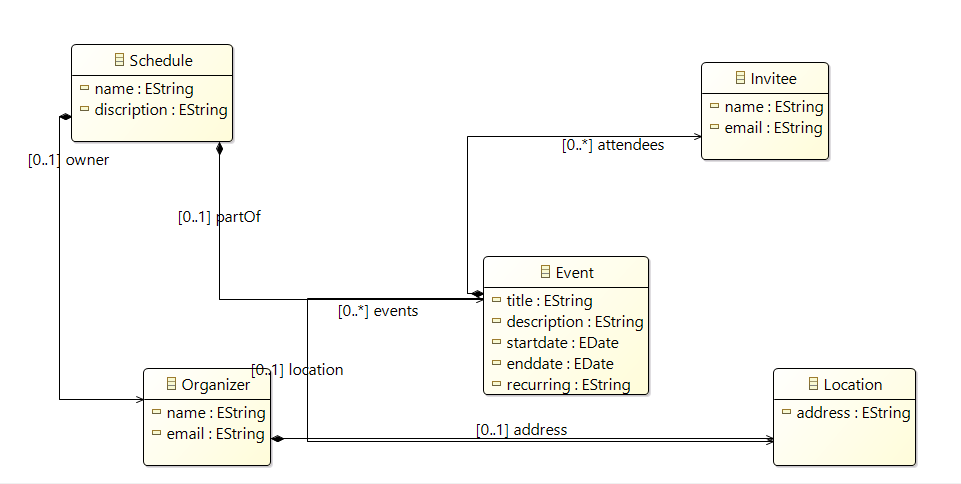
\includegraphics[width=0.7\textwidth]{class.png}
    \caption{Class Diagram of the ICS Helper DSL Metamodel}
    \label{fig:class-diagram}
\end{figure}

The diagram illustrates the associations between the main entities, providing a visual reference for the metamodel.

This metamodel analysis and class diagram form the basis for the subsequent development and implementation of the ICS Helper DSL.


\newpage
\section{Defining and Implementing Syntax}
We choose Xtext to implement the syntax and generate editor accordingly for the below reasons:

\begin{itemize}
    \item Xtext, as a text-based tool, provide flexible syntax control.
    \item Consider the use case of our dsl, usability in a text-based environment is a must.
    \item Better integration with other platforms and tools.
\end{itemize}

\subsection{Syntax}
Aiming to be user-friendly and intuitive, the syntax of ICS Helper DSL is designed to be concise and natural-language-like. 
The following sections outline the syntax elements and examples of the DSL.
\subsubsection{Basic Syntax}
\begin{verbatim}
    'create' 'schedule' UNIQUE_NAME '{'
        one or more Event
    '}'
\end{verbatim}

Where \texttt{Event} is defined as follows:

\begin{verbatim}
    'event' UNIQUE_NAME
    'start' YYYY-MM-DD HH:MM:SS
    'end' YYYY-MM-DD HH:MM:SS
    (OPTIONAL FIELDS)
\end{verbatim}
OPTIONAL FIELDS include: \texttt{location}, \texttt{description}, \texttt{organizer}, \texttt{invitees}, \texttt{recurrence rule}, \texttt{reminder rule}, \texttt{link}. 
Please refer to our documentation for more details.

\subsubsection{example}
\begin{figure}[H]
    \centering
    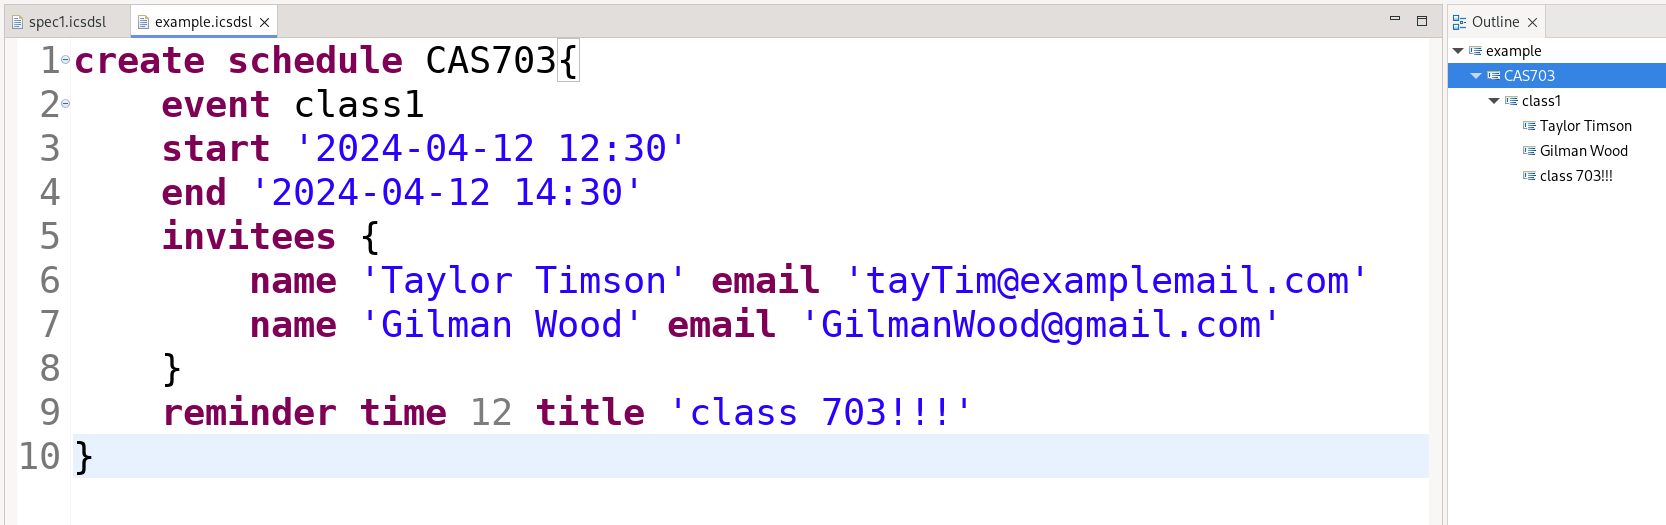
\includegraphics[width=0.7\textwidth]{editor_example.png}
    \caption{Example Editor Screenshot}
    \label{fig:class-diagram}
\end{figure}

\begin{verbatim}
    create schedule CAS703{
        event class1 
        start '2024-04-12 12:30'
        end '2024-04-12 14:30'
        invitees {
            name 'Taylor Timson' email 'tayTim@examplemail.com'
            name 'Gilman Wood' email 'GilmanWood@gmail.com'
        }
        reminder time 15 title 'go to class 703!!!'
    }
\end{verbatim}

\subsection{Discussion}
Our syntax design using Xtext comes with the following advantages:
\begin{itemize}
    \item Friendly syntax that is easy to understand and use.
    \item Editor that provides syntax highlighting, auto-completion, and error checking.
    \item Portability and integration with other tools (as our project is shipped as a plugin). 
\end{itemize}
At the same time, it comes with the following limitations:
\begin{itemize}
    \item Dependence on the Eclipse environment.
    \item Grammar limitations: like the need to follow the time format exactly, which hinders easy-usage.
    \item Higher learning curve compared to graphical editors.
\end{itemize}


\newpage
\section{Validation constraints implementation}
Erin's part

Following lists the implementation of each constraints using Epsilon Validation Languag (EVL).
\begin{itemize}
    \item ICSFile: The file name and content cannot be null or empty.    
    \item schedule:The schedule name cannot be null or empty.
    \item Event:The event name cannot be null or empty. 
\end{itemize}

\newpage
\section{Model management operation implementation}
Ahila
% Uncomment following to add an acknowledgement section
% \section*{Acknowledgements}

% Thanks again to \textbf{Person 1} and \textbf{Affiliation A} for their financial support.

% ----------
% Bibliography
% ----------

% Uncomment the following and add your references into biblio.bib file
% \bibliography{./biblio.bib}
% \bibliographystyle{abbrv}

\section{References}

\end{document}

% ----------